\documentclass[12pt]{article}

% Layout.
\usepackage[top=1in, bottom=0.75in, left=1in, right=1in, headheight=1in, headsep=6pt]{geometry}

% Fonts.
\usepackage{mathptmx}
\usepackage[scaled=0.86]{helvet}
\renewcommand{\emph}[1]{\textsf{\textbf{#1}}}

% TiKZ.
\usepackage{tikz, pgfplots}
\usetikzlibrary{calc}
\pgfplotsset{compat = newest}
 
\pgfplotsset{my style/.append style={axis x line=middle, axis y line=
middle, xlabel={$x$}, ylabel={$y$}, axis equal }}

% Misc packages.
\usepackage{amsmath,amssymb,latexsym}
\usepackage{graphicx}
\usepackage{array}
\usepackage{xcolor}
\usepackage{multicol}

% Commands to set various header/footer components.
\makeatletter
\def\doctitle#1{\gdef\@doctitle{#1}}
\doctitle{Use {\tt\textbackslash doctitle\{MY LABEL\}}.}
\def\docdate#1{\gdef\@docdate{#1}}
\docdate{Use {\tt\textbackslash docdate\{MY DATE\}}.}
\def\doccourse#1{\gdef\@doccourse{#1}}
\let\@doccourse\@empty
\def\docscoring#1{\gdef\@docscoring{#1}}
\let\@docscoring\@empty
\def\docversion#1{\gdef\@docversion{#1}}
\let\@docversion\@empty
\makeatother

% Headers and footers layout.
\makeatletter
\usepackage{fancyhdr}
\pagestyle{fancy}
\fancyhf{} % Clears all headers/footers.
\lhead{\baselineskip 30pt
%\emph{\@doctitle\hfill\@docdate}
\emph{\@docdate\hfill\@doctitle}
\ifnum \value{page} > 1\relax\else\\
\emph{Name: \rule{3.5in}{1pt}\hfill \@docscoring}\fi}
\rfoot{\emph{\@docversion}}
\lfoot{\emph{\@doccourse}}
\cfoot{\emph{\thepage}}
\renewcommand{\headrulewidth}{0pt}%
\makeatother

% Paragraph spacing
\parindent 0pt
\parskip 6pt plus 1pt

% A problem is a section-like command. Use \problem{5} to
% start a problem worth 5 points.
\newcounter{probcount}
\newcounter{subprobcount}
\setcounter{probcount}{0}
\newcommand{\problem}[1]{%
\par
\addvspace{4pt}%
\setcounter{subprobcount}{0}%
\stepcounter{probcount}%
\makebox[0pt][r]{\emph{\arabic{probcount}.}\hskip1ex}\emph{[#1 points]}\hskip1ex}
\newcommand{\thesubproblem}{\emph{\alph{subprobcount}.}}

% Subproblems are an enumerate-like environment with a consistent
% numbering scheme. 
% Use \begin{subproblems}\item...\item...\end{subproblems}
\newenvironment{subproblems}{%
\begin{enumerate}%
\setcounter{enumi}{\value{subprobcount}}%
\renewcommand{\theenumi}{\emph{\alph{enumi}}}}%
{\setcounter{subprobcount}{\value{enumi}}\end{enumerate}}

% Blanks for answers in normal and math mode.
\newcommand{\blank}[1]{\rule{#1}{0.75pt}}
\newcommand{\mblank}[1]{\underline{\hspace{#1}}}
\def\emptybox(#1,#2){\framebox{\parbox[c][#2]{#1}{\rule{0pt}{0pt}}}}

% Misc.
\renewcommand{\d}{\displaystyle}
\newcommand{\ds}{\displaystyle}
\def\bc{\begin{center}}
\def\ec{\end{center}}
\def\be{\begin{enumerate}}
\def\ee{\end{enumerate}}


\doctitle{Math 251: Quiz 10}
\docdate{Fall 2025}
\doccourse{UAF Calculus I}
\docversion{v-1}
\docscoring{\blank{0.8in} / 25}
\begin{document}
%\textbf{Please circle your instructor's name:} \hfill Kevin Meek \hfill James Gossell \hfill Margaret Short \\

There are 25 points possible on this quiz. No aids (book, calculator, etc.)
are permitted.  {\bf Show all work for full credit.}


\problem{3} For the function $\displaystyle F(x)=\int_3^{x^2} \sqrt{t} \: dt$, use the Fundamental Theorem of Calculus to find $F'(x)$.\\
	
	\vspace{0.5in}
	$F'(x)=$
	\vspace{0.3in}

\problem{9} Evaluate the definite integrals below. Use proper notation and simplify your answers.
\begin{subproblems}
\item $\displaystyle \int_{0}^{2} (3e^x+2) \: dx$
\vfill
\item $\ds \int_1^3 t(t-2) \;\, dt$ 
\vfill
\item $\displaystyle \int_{0}^{\pi} \left(2\sin(x)+3\cos(x)\right) \: dx$
\vfill
\end{subproblems}

\newpage

\problem{8} Evaluate the following indefinite integrals (antiderivatives) below. Clearly state any substitutions you use and write your final answer in terms of $x$.
\begin{subproblems}
\item $\ds \int \frac{\sin(\ln(x))}{x}\; dx$	
\vfill
\item $\ds\int \frac{-3x^2+\sin(x)}{x^3+\cos(x)} \; dx$
\vfill
\end{subproblems}


\problem{5} Use the graph of $f(x)$ (below) to answer questions about $\displaystyle A(x)= \int_{-5}^x f(t) \: dt.$

\begin{multicols}{2}
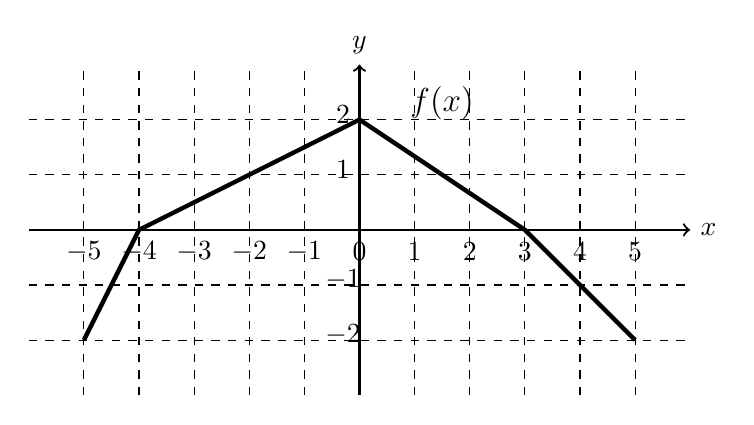
\begin{tikzpicture}[scale = .7]
% axes
\draw[thick, ->] (-6,0) -- (6,0) node[right]{$x$};
\draw[thick, ->] (0,-3) -- (0,3) node[above]{$y$};

% graph: piecewise linear with integer x-intercepts
% segments: (-5,-2) to (-4,0) to (0,2) to (3,0) to (5,-2)
\draw[ultra thick] (-5,-2) -- (-4,0) -- (0,2) -- (3,0) -- (5,-2);

% vertical dashed lines and labels
\foreach \x in {-5,-4,-3,-2,-1,0,1,2,3,4,5}{
  \draw[dashed] (\x,-3) -- (\x,3);
  \node at (\x,-0.4) {$\x$};
}

% horizontal dashed lines
\foreach \y in {-2,-1,1,2}{
  \draw[dashed] (-6,\y) -- (6,\y);
  \node at (-0.3,\y+0.1) {$\y$};
}

\node at (1.5,2.3) {\large $f(x)$};

\end{tikzpicture}
\vspace{.6in}
\columnbreak
\begin{subproblems}
	\item $A(-2)= $\ \blank{1cm}
	\item $A(4)=$\ \blank{1cm}
	\item $A'(0) = $\ \blank{1cm}
	\item On the interval $[-5,5]$, where does $A(x)$ have a maximum or minimum?\\
	
	Maximum at $x = $\  \blank{1cm}\\
	
	Minimum at $x = $\  \blank{1cm}

	\vspace{2cm}
\end{subproblems}
\end{multicols}
	
\end{document}
%%% Local Variables:
%%% mode: LaTeX
%%% TeX-master: t
%%% End:
